\documentclass[pdftex]{book}
\usepackage[papersize={4in, 4in},top=0.1in,bottom=0.1in,left=0.1in,right=0.1in]{geometry}
\usepackage{pgfplots}
\usepgfplotslibrary{fillbetween}
\renewcommand{\familydefault}{\sfdefault}
\begin{document}
\thispagestyle{empty}
\begin{center}
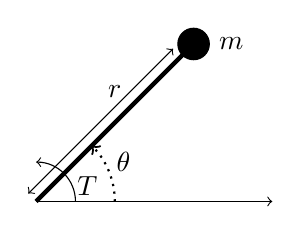
\begin{tikzpicture}[scale=2]
\draw [fill] (1,1) circle [radius=0.1];
\draw [->] (0, 0) -- (1.5,0);
\draw [ultra thick] (0, 0) -- (1, 1);
\draw [thick, dotted, ->] (0.5,0) arc (0:45:0.5);
\draw [->] (0.25,0) arc (0:90:0.25);
\draw [<->] (-0.05,0.05) -- (0.87,0.97);
\node [right] at (0.45,0.25) {$\theta$};
\node [right] at (0.2,0.1) {$T$};
\node [right] at (1.1,1.0) {$m$};
\node[above] at (0.5,0.6) {$r$};
\end{tikzpicture}
\end{center}
Assume a point mass $m$ at radius $r$ from a pivot point attached by a massless arm with length $r$.
The angle of the arm is $\theta$, a function of time.
The torque applied to the arm is $T$, positive in the counterclockwise direction.
The moment of inertia is given by
\[
I = m r^2 .
\]
The angular version of Newton's second law is
\[
T = I \ddot{\theta} .
\]
The torque due to gravity is given by
\[
T_g = - mrg \cos(\theta),
\]
where $g = 9.81$ m/s$^2$ is the acceleration of gravity at sea level.
The net torque is $T-T_g$.
Hence,
\[
\ddot{\theta} = \frac{T}{mr^2} - \frac{g \cos(\theta)}{r} .
\]
\end{document}